\documentclass[10pt]{article}
\usepackage{amsmath, amsfonts, amssymb, amsthm}
\usepackage[colorlinks=true, allcolors=blue]{hyperref}
\usepackage{tikz}
\usepackage{xcolor}
\usepackage{pgfplots}

\begin{document}

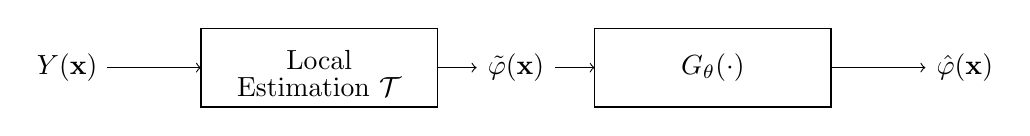
\begin{tikzpicture}
\node at (-1.7, 0.0) {$Y(\mathbf{x})$};
\draw [->] (-1.2, 0.0) -- (0, 0.0);
\draw (0,-0.5) rectangle (3, 0.5);
\node at (1.5, 0.1) {Local};
\node at (1.5, -0.25) {Estimation $\mathcal{T}$};
\draw [->] (3, 0.0) -- (3.5, 0.0);
\node at (4.0, 0.0) {$\tilde{\varphi}(\mathbf{x})$};
\draw [->] (4.5, 0.0) -- (5, 0.0);
\draw (5, -0.5) rectangle (8, 0.5);
\node at (6.5, 0.0) {$G_\theta(\cdot)$};
\draw [->] (8, 0.0)--(9.2, 0.0);
\node at (9.7, 0.0) {$\hat{\varphi}(\mathbf{x})$};   
\end{tikzpicture}

\end{document}